\chapter{Características generales del diseño}
\section{Objetivos globales del sistema}

En base a la información recolectada establecemos los requerimientos base del que se parte para el diseño del producto final. Creemos adecuado
realizar la separación de requerimientos en primarios y secundarios, ya que el sistema a desarrollar está enmarcado en el proyecto final de la 
carrera de grado de ingeniería electrónica donde, en conjunto con la cátedra, se intenta que los proyectos puedan culminarse en un plazo de 
tiempo lógico para la obtención del título, dando la posibilidad de seguir explayándose en el mismo a posterior. \par

De este modo, como objetivos primarios se establecen:

\begin{itemize}
    \item Identificar la presencia de señales con una potencia suficiente para inhibir la comunicación: como en el marco teórico se ha 
    estudiado en profundidad, la etapa amplificadora receptora sufre una compresión de la ganancia cuando en su entrada hay presente 
    una señal de alto nivel de potencia. Es por esto que se establece como requerimiento del sistema poder identificar una señal que cumpla con
    estas características.
    \item Medir la ocupación del canal: Ha quedado claro que la trama de comunicación de las llaves remotas con los receptores de los automóviles 
    poseen características de espaciado entre paquetes de datos transmitidos, es por esto que el sensado de la ocupación del canal se vuelve 
    una medida crucial para determinar si hay o no presencia de interferencias.
    \item Activar alarmas sonoras y visuales en caso de estar en presencia de una inhibición: el sistema debe tener la capacidad de determinar 
    si hay presente una inhibición en su área de operación y, de ser así, debe disponer de métodos para dar alerta local de lo que está sucediendo.
    \item Disponer de comunicación a sistemas externos complementarios: un requisito del sistema es que posea la capacidad de enviar la información recolectada
    a un lugar remoto. Se prefiere la utilización de una metodología de comunicación inalámbrica y ampliamente distribuida.
    \item Cargar los datos en una base de datos: es importante que la información de las inhibiciones detectadas sea subida a una base de datos
    que permita visualizar de manera remota y en tiempo real lo que está sucediendo con los sistemas de seguridad activos, brindando la posibilidad 
    de generar estadísticas y observar qué tipos de inhibidores están operando en la zona.
    \item Orientar el diseño del proyecto a la optimización de costos y recursos: es muy importante para el curso del trabajo que el diseño 
    se realice haciendo uso racional de los recursos disponibles, apuntando a la posibilidad de producir muchas unidades del sistema de seguridad
    y obtener ganancias.

\end{itemize}

Como objetivo secundario se define:

\begin{itemize}
    \item Estimar la procedencia de la interferencia: el único objetivo secundario del sistema es que tenga la capacidad, mediante el método 
    más conveniente, de determinar la posición estimada de la fuente de interferencia activa. Esto está planteado de esta manera debido a que 
    se desconoce la factibilidad de su realización en el marco del proyecto de fin de grado de ingeniería electrónica.
\end{itemize}

\section{Esquema de funcionamiento}

En la figura \ref{bloques_funcionamiento} se puede observar el sistema planteado para solucionar el desafío de detectar inhibiciones en los sistemas
de seguridad vehicular. El mismo contará con nodos detectores que operarán en 433,92 MHz, un canal de comunicación hacia la central, haciendo
uso de un protocolo que más adelante se detallará y una central de operación donde se decidirá si hay o no inhibición en su área de operación
desatando las alarmas pertinentes y subiendo la información al servidor. \par

\begin{figure}[htb]
	\centering
	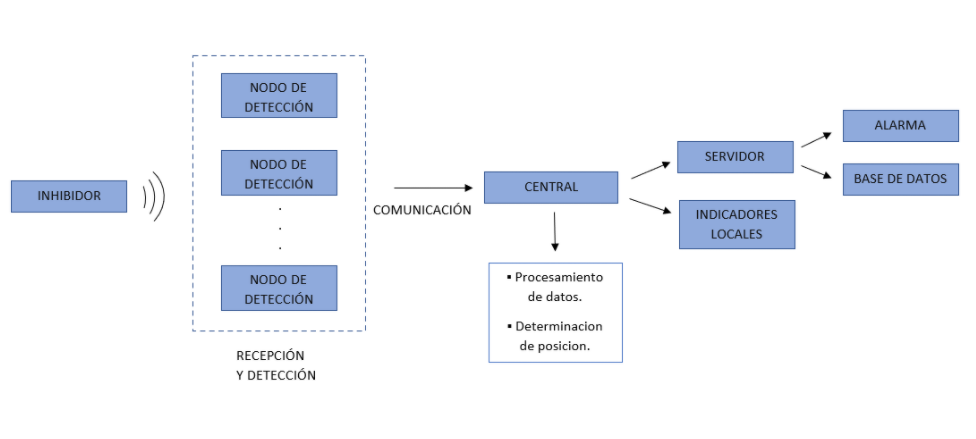
\includegraphics[scale=0.53]{images/bloques_funcionamiento.png}
    \caption{Diagrama en bloques sobre el funcionamiento del sistema global}
	\label{bloques_funcionamiento}
\end{figure}

\section{Subsistemas que lo componen}

En esta sección únicamente se hará mención de los subsistemas que componen al producto final, más adelante se detallará en capítulos el funcionamiento 
particular de cada uno de estos bloques.

\begin{itemize}
    \item Nodo receptor 
    \begin{itemize}
          \item Microcontrolador STM32F103C8T6.
          \item Receptor de RF. 
          \item Integrado para comunicación RS-485.
    \end{itemize}
    \item Central de procesamiento 
    \begin{itemize}
          \item Microcontrolador STM32F103C8T6.
          \item Integrado para comunicación GSM/GPRS. 
          \item Integrado para comunicación RS-485.
    \end{itemize}
    
\end{itemize}
